% !TEX encoding = UTF-8 Unicode
%!TEX root = thesis.tex
% !TEX spellcheck = en-US
%%=========================================
\chapter{Results}

The results will be introduced in the same order as the experiments were conducted. First, the results of matching of one of the EDX datasets with the SPED dataset will be presented. This is followed the position matching of the various EDX datasets with the overview images. Lastly, the calculated $\zeta$-factors and the quantification of the samples using the $\zeta$-factor method and the Cliff-Lorimer technique are displayed.

\section{Dataset matching}

\cref{fig:edxsped} shows the results of matching the largest EDX dataset with the SPED dataset. \cref{fig:edxspedorig} shows the first result, with the SPED dataset rotated by the manually estimated angle, and the EDX dataset scaled using the scale factor obtained from the metadata. In \cref{fig:edxspedrot}, the angle has been iteratively optimized, and therefore increased by 0.4\% (0.4 $\deg$). \cref{fig:edxspedscale} shows the third result, where only the scale factor has been optimized. The lowest matching value was found if the scale factor was reduced by 6.5\%. The final attempt, in which both the rotation angle and the scale factor were iterated, resulted in the angle being increased by 2.8\% (2.6 $\deg$) which was clearly too much. Should processed images be shown as well? %\cref{fig:edxspedboth1} also shows the third result, but here with the processed images.
In \cref{fig:edxspedorig,fig:edxspedrot} the results are very similar, and it appears from the nanowire that the EDX image is larger than the SPED image. In \cref{fig:edxspedscale}, on the other hand, the EDX image appears slightly smaller than the SPED image. 
% As explained in \cref{sec:method/dataset matching}, these images have been processed to be made more similar. \cref{fig:edx-in-sped-edx} shows the EDX image and \cref{fig:edx-in-sped-rectangle} shows the SPED image with a rectangle indicating where the best fit of the EDX image was found. 

\begin{figure}
	\centering
	\begin{subfigure}{0.25\textwidth}
		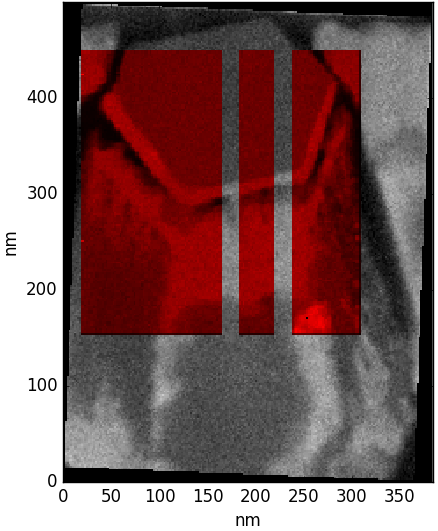
\includegraphics[width=\textwidth]{fig/other/edxinsped/orig5-2}
		\caption{}
		\label{fig:edxspedorig}
	\end{subfigure}%
	\hfill
	\begin{subfigure}{0.25\textwidth}
		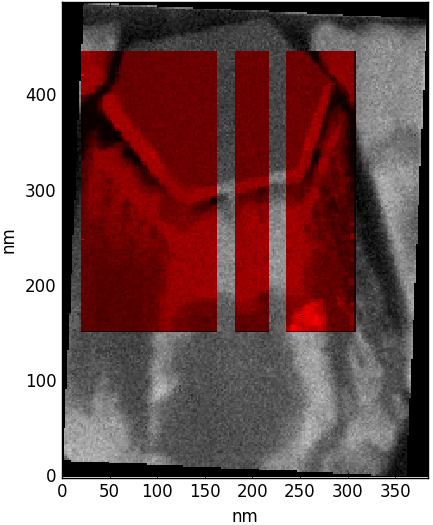
\includegraphics[width=\textwidth]{fig/other/edxinsped/rot5-2}
		\caption{}
		\label{fig:edxspedrot}
	\end{subfigure}%
	\begin{subfigure}{0.25\textwidth}
		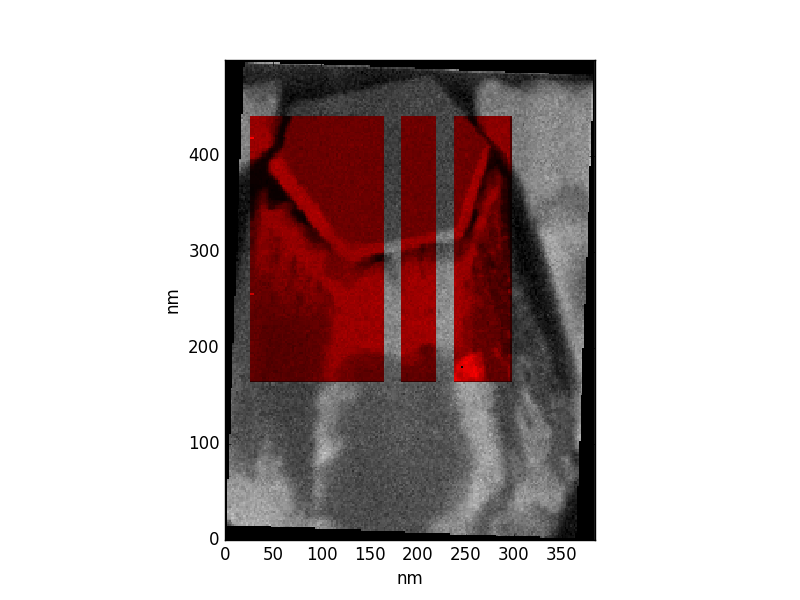
\includegraphics[width=\textwidth]{fig/other/edxinsped/show/onlyScale}
		\caption{}
		\label{fig:edxspedscale}
	\end{subfigure}%
%	\begin{subfigure}{0.25\textwidth}
%	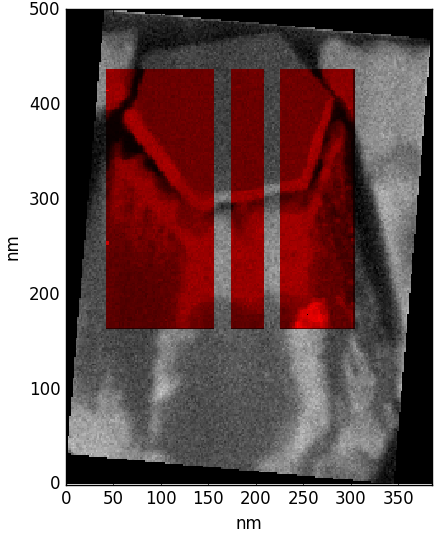
\includegraphics[width=\textwidth]{fig/other/edxinsped/show/both1-2}
%	\caption{}
%	\label{fig:edxspedboth1}
%	\end{subfigure}
%	\hfill
%	\begin{subfigure}{0.25\textwidth}
%		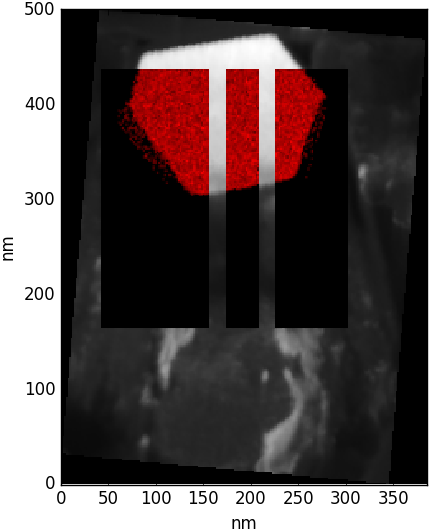
\includegraphics[width=\textwidth]{fig/other/edxinsped/show/both2-2}
%		\caption{}
%		\label{fig:edxspedboth2}
%	\end{subfigure}%
	\caption{
		\label{fig:edxsped}%
		Caption}
\end{figure}


%\begin{figure}
%\begin{subfigure}{.5\textwidth}
%	\centering
%	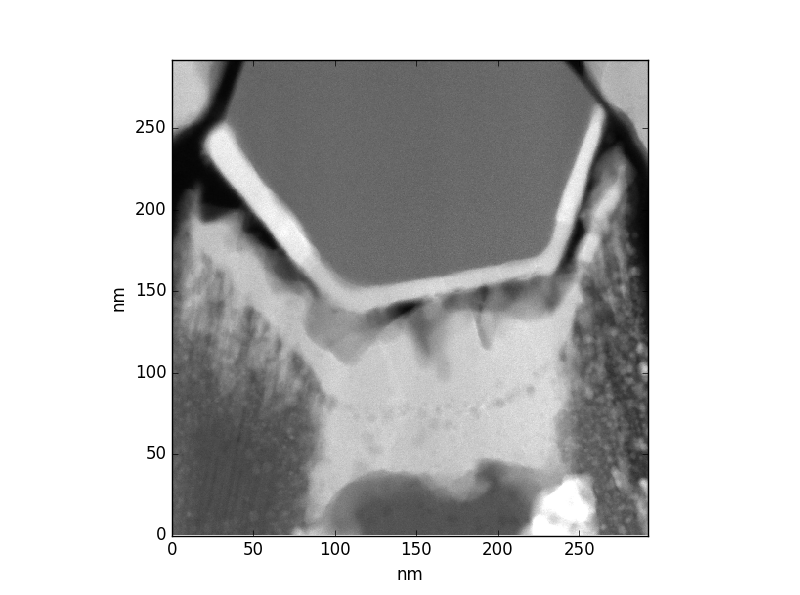
\includegraphics[width=\linewidth]{fig/in-rectange}
%	\caption{++++++}
%	\label{fig:edx-in-sped-edx}
%\end{subfigure}%
%\begin{subfigure}{.5\textwidth}
%	\centering
%	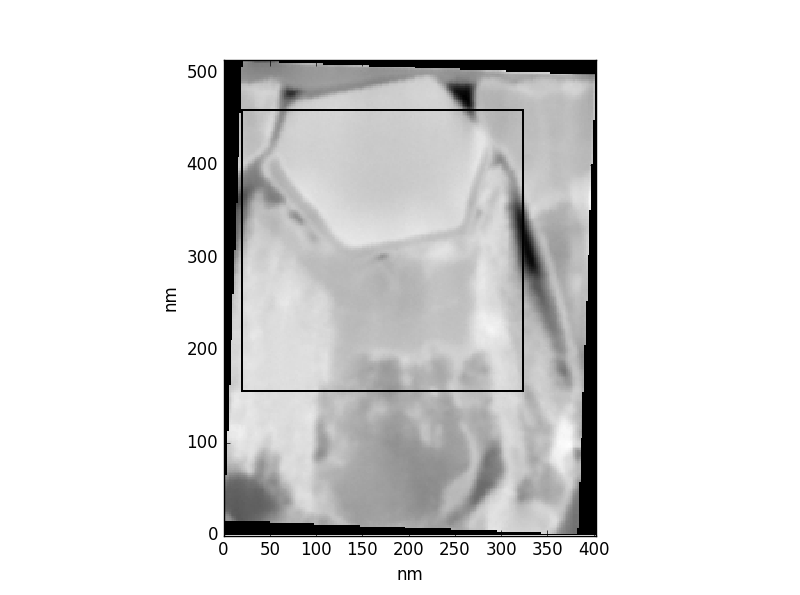
\includegraphics[width=\linewidth]{fig/sdrot-with-rectange}
%	\caption{++++++}
%	\label{fig:edx-in-sped-rectangle}
%\end{subfigure}
%\caption{plots of....}
%\label{fig:edx-in-sped}
%\end{figure}

%As the correct result is unknown, it is difficult to quantify the error in the fit. An attempt was made by looking at the difference between the matching value for the best position, shown in \cref{fig:edx-in-sped-rectangle}, and the higher values. The matching values are defined in \cref{eq:matching value}. \cref{fig:edx-sped-rectangle-match-graph} shows the relative error of the 100 best matching values with respect to the best match. 

%\begin{figure}
%	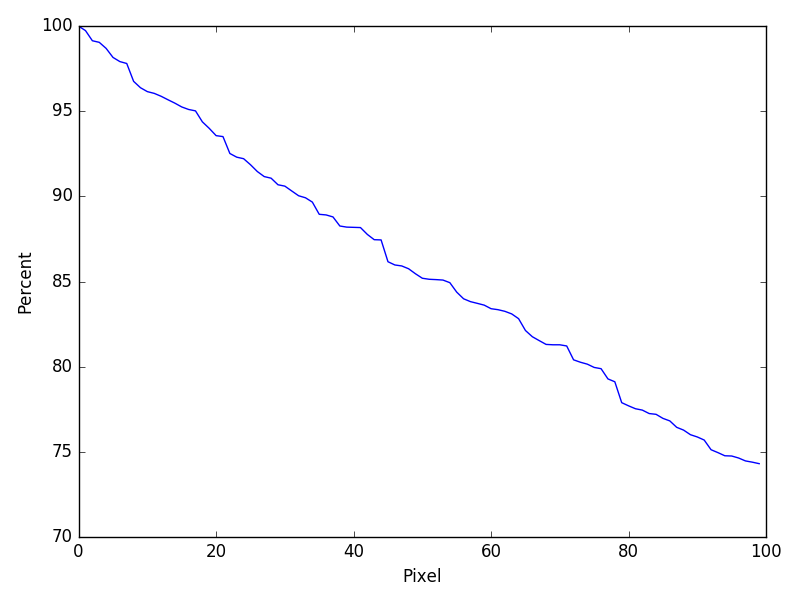
\includegraphics[width=0.7\linewidth]{fig/edx-sped-rectangle-match-graph.png}
%	\caption{++++++}
%	\label{fig:edx-sped-rectangle-match-graph}
%\end{figure}

The results from locating the EDX datasets in the HAADF overview images are displayed in \cref{fig:nonheated-images-in-overview, fig:heated-images-in-overview} for the non-treated and the heat-treated samples, respectively. In the non-treated sample, the two datasets B and D were not correctly located in the overview image. The calculated location of dataset B was completely off, while the position of D was just slightly offset. The actual positions of these datasets were estimated by eye and marked in \cref{fig:nonheated-images-in-overview} as blue dotted rectangles. The rest of the datasets were located correctly, and their positions are shown as red rectangles. For the heat-treated sample, all the datasets that were included in the overview image were correctly located. However, the areas covered by two the datasets A and B were found to not be included in the overview image.


\begin{figure}
	\begin{subfigure}{.5\textwidth}
		\centering
		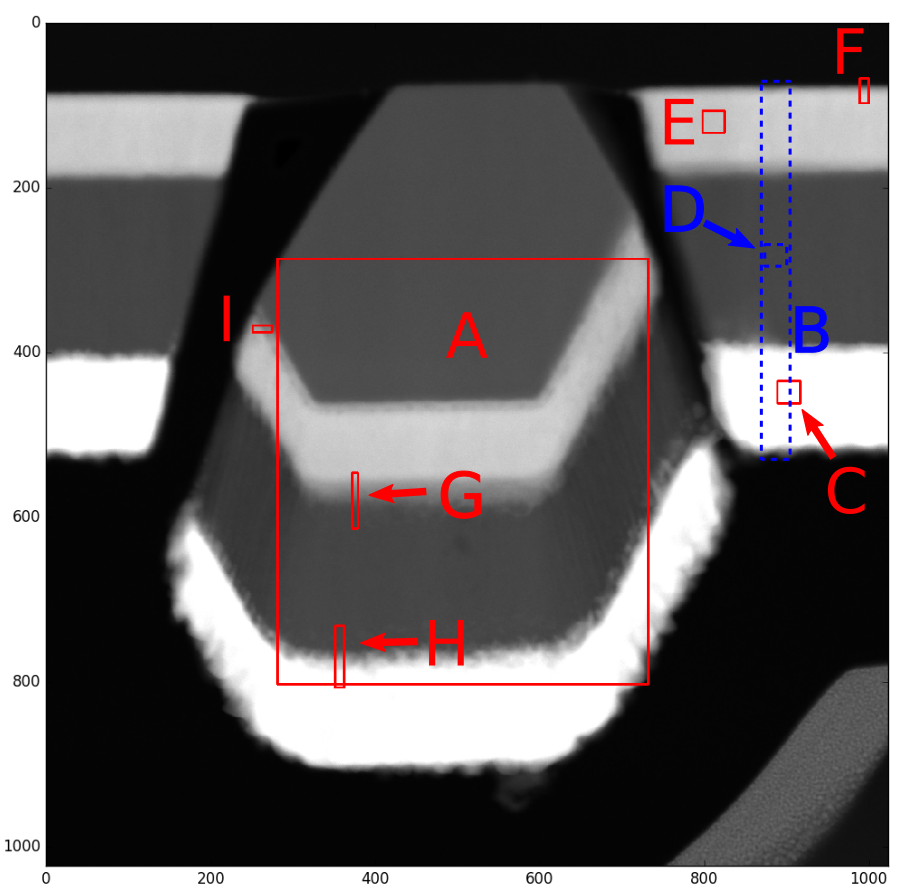
\includegraphics[width=\linewidth]{fig/nonheated-img-in-overview}
		\caption{}
		\label{fig:nonheated-images-in-overview}
	\end{subfigure}%
	\begin{subfigure}{.5\textwidth}
		\centering
		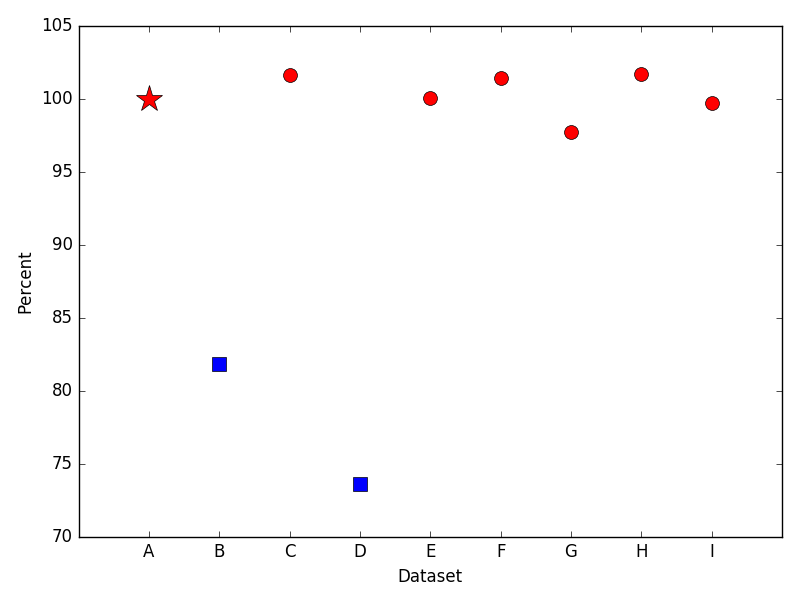
\includegraphics[width=\linewidth]{fig/nonheated-matching-values}
		\caption{}
		\label{fig:nonheated-matching-values}
	\end{subfigure}
	\caption{Nonheated edx in sped}
	\label{fig:nonheated-overview}
\end{figure}

\begin{figure}
	\begin{subfigure}{.5\textwidth}
		\centering
		\includegraphics[width=\linewidth]{"fig/heated-images-in-overview-ink2"}
		\caption{}
		\label{fig:heated-images-in-overview}
	\end{subfigure}%
	\begin{subfigure}{.5\textwidth}
		\centering
		\includegraphics[width=\linewidth]{"fig/heated-matching-values"}
		\caption{}
		\label{fig:heated-matching-values}
	\end{subfigure}
	\caption{Heated edx in sped}
	\label{fig:heated-overview}
\end{figure}

The accuracy of the matching for the different datasets are shown in \cref{fig:nonheated-matching-values} for the non-heated sample, and in \cref{fig:heated-matching-values} for the heated values. The horizontal axis shows the different datasets while the vertical axis is the matching value in percent, where 100 \% is defined to be the matching value of the dataset covering the biggest area in each respective sample. The matching of this dataset is assumed to be the most trustworthy due to there being fewer potential locations that resemble the actual location, as there are several distinct features. For the smaller datasets, or more accurately, the datasets with smaller survey images, there might be several different locations in the overview image that all give a fairly good match.

In both figures, the red star is the value of the dataset used as reference, the red circles are the correctly matched datasets while the blue squares are the datasets that resulted in a wrong location. The non-heated sample (\cref{fig:nonheated-matching-values}) shows high values for all the correctly located datasets, and significantly lower values for the wrongly located ones. In addition, it must be noted that the exact location of dataset F was impossible to verify visually due to the survey image not being large enough to distinguish specific features. In the heated sample (\cref{fig:heated-matching-values}), all the red correctly located datasets have high values while the datasets that were not present in the reference image have distinguishably lower values.

\section{Determination of $\zeta$-values}

The calculated $\zeta$-values for all the characteristic X-ray lines used to quantify the data are presented in \cref{tab:non-heated zeta-values}, along with which dataset was used to calculate them. The calculated $\zeta$-values were compared to the corresponding $k$-values using \cref{compare_zeta_CL}, with Ga$_{K\alpha}$ as reference element. \cref{fig:zeta-k-comparison} shows the results, with the mean value and spread of the $\zeta$-factors indicated. The average $\zeta$-values have been used for all further calculations. 

%\begin{table}[h!]
%	\caption{zeta values}
%	\begin{center}
%	\begin{tabular}{ccccc}
%
%	Element & Dataset & $K_\alpha$ & $L_\alpha$ & $M_\alpha$ \\ 
%	\midrule
%	\hline
%	Ga ($K_\alpha$)  & C* & 582\\
%	Ga ($K_\alpha$)  & A  & 608\\ \hline
%	As ($K_\alpha$)  & C* & 689\\
%	As ($K_\alpha$)  & A  & 706\\ \hline
%	Ge ($K_\alpha$)  & B  & 732\\
%	Ge ($K_\alpha$)  & D  & 741\\
%	Ge ($K_\alpha$)  & A  & 748\\ \hline
%	Ge ($L_\alpha$)  & A  & 933\\
%	Ge ($L_\alpha$)  & D  & 900\\
%	Ge ($L_\alpha$)  & B  & 900\\ \hline
%	Pd ($L_\alpha$)  & E  & 1248\\
%	Pd ($L_\alpha$)  & A  & 1284\\
%	Pd ($L_\alpha$)  & B  & 1318\\ \hline
%%	AuL & B  & 3450\\ 
%%	AuL & C  & 3473\\
%	Au ($M_\alpha$) & B & 2397\\
%	Au ($M_\alpha$) & C & 2387\\
%	\hline
%	\end{tabular}
%	\end{center}
%	\label{tab:non-heated zeta-values}
%\end{table}

\begin{table}[h!]
	\caption{zeta values}
	\begin{center}
		\begin{tabular}{ccccc}
			Element & Dataset & $K_\alpha$ & $L_\alpha$ & $M_\alpha$ \\ 
			\midrule
			\hline
			Ga  & C* & 486 & 512 & -\\
			Ga  & A  & 608 & 826 & -\\ \hline
			As  & C* & 576 & 600 & -\\
			As  & A  & 706 & 955 & -\\ \hline
			Ge  & B  & 729 & 898 & -\\
			Ge  & D  & 740 & 901 & -\\
			Ge  & A  & 745 & 933 & -\\ \hline
			Pd  & E  & - & 1249 & -\\
			Pd  & A  & - & 1284 & -\\
			Pd  & B  & - & 1316 & -\\ \hline
			Au  & B  & - & 3422 & 2396\\
			Au  & C  & - & 3426 & 2387\\
			\hline
		\end{tabular}
	\end{center}
	\label{tab:non-heated zeta-values}
\end{table}


\begin{figure}[h]
	\centering
	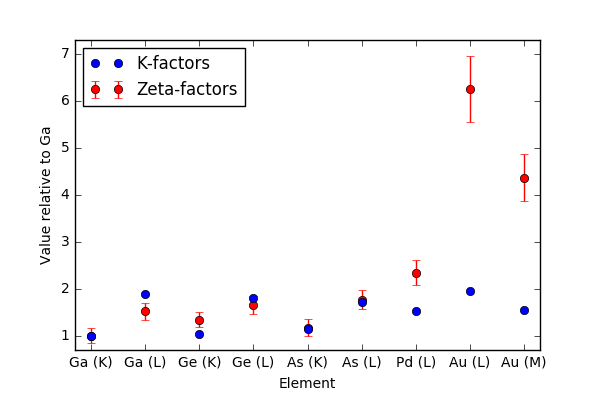
\includegraphics[width=0.7\linewidth]{fig/other/zeta-k-plot-new}
	\caption{zeta - k - comparison}
	\label{fig:zeta-k-comparison}
\end{figure}

\section{Quantification}

%Secondly, when attempting to calculate the composition of Ga and As simultaneously with Au, the results were very bad. Thirdly, if measuring the composition of Ga and As simultaneously with Ge, using the Ge\_{L$\alpha$}-peak, all three techniques said there was 10\% Ge in the area known to consist of only Ga and As. This did not happen while using the Ge\_{K$\alpha$}-peak. To conclude, when measuring elements Ga, As, Ge and Pd, the Ge\_{K$\alpha$}-peak was used, but when measuring elements Ge, Pd and Au, the Ge\_{L$\alpha$}-peak was used.

\cref{fig:zeta_area1,fig:zeta_area2} shows the compositions of two areas (\cref{fig:zeta_area1_overview,fig:zeta_area2_overview} shows the locations of these areas) in the untreated sample, as calculated using the Cliff-Lorimer ratio method (CL method) and the $\zeta$-factor method with and without absorption correction. All the spectra have been averaged in the horizontal direction. The results are as expected. \cref{fig:zeta_area1_ga,fig:zeta_area1_as} shows that the nanowire consists of Ga and As in a 50:50 ratio, and \cref{fig:zeta_area1_ge,fig:zeta_area1_pd} shows that the next two layers are approximately 100\% Pd and 100\% Ge, respectively. In the second area, \cref{fig:zeta_area2_pd,fig:zeta_area2_ge,fig:zeta_area2_au} shows that the composition of elements are approximately 100\% Au in the top region, 100\% Pd in the middle and 100\% Ge in the lower region.

All three techniques give fairly similar answers for Ga and As, while the differences between the CL- and $\zeta$-factor methods are significantly higher for Pd, Ge and Au. The inclusion of absorption correction does not give very different results for any of the elements, except for the Ge-region in the second area where the absorption correction appears to significantly amplify two erroneous peaks.
%\cref{fig:zeta_area1_all,fig:zeta_area2_all} shows the compositions of all the element as calculated using the $\zeta$-method with absorption correction. 
There is a clear transitioning length between each of the elements layers where the spectra shows characteristic peaks belonging to both elements. This length is shortest for the transition between GaAs and Pd, and longest between Pd and Ge.

\begin{figure}
	\begin{subfigure}{.5\textwidth}
		\centering
		\newlength\imageheight
		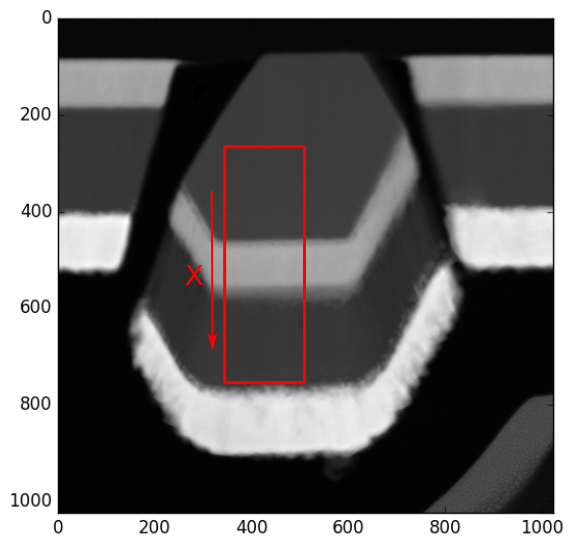
\includegraphics[width=.68\linewidth]{fig/q/1_overview3}
		\caption{}
		\label{fig:zeta_area1_overview}
	\end{subfigure}
	\begin{subfigure}{.45\textwidth}
		\centering
		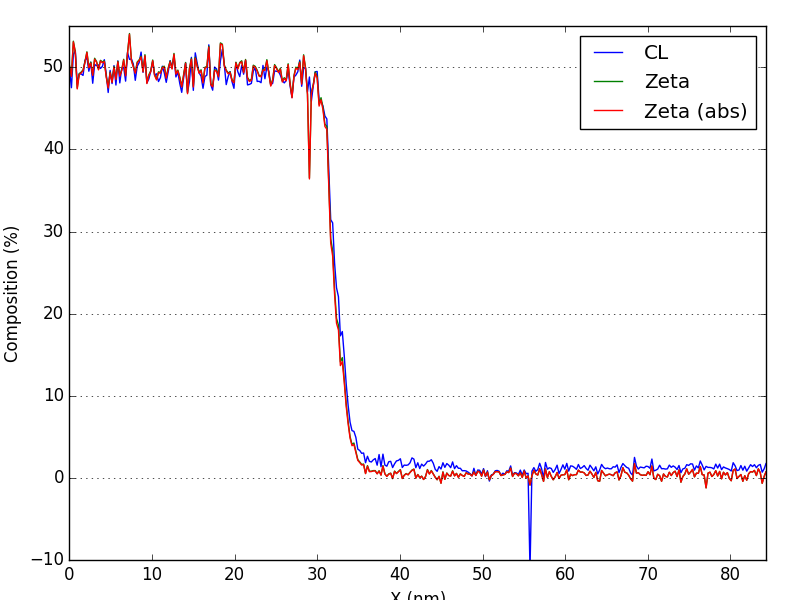
\includegraphics[width=\linewidth]{fig/q-new/oldzetas_Sa_Ga_Ka}
		\caption{}
		\label{fig:zeta_area1_ga}
	\end{subfigure}%
\hfill
	\begin{subfigure}{.45\textwidth}
		\centering
		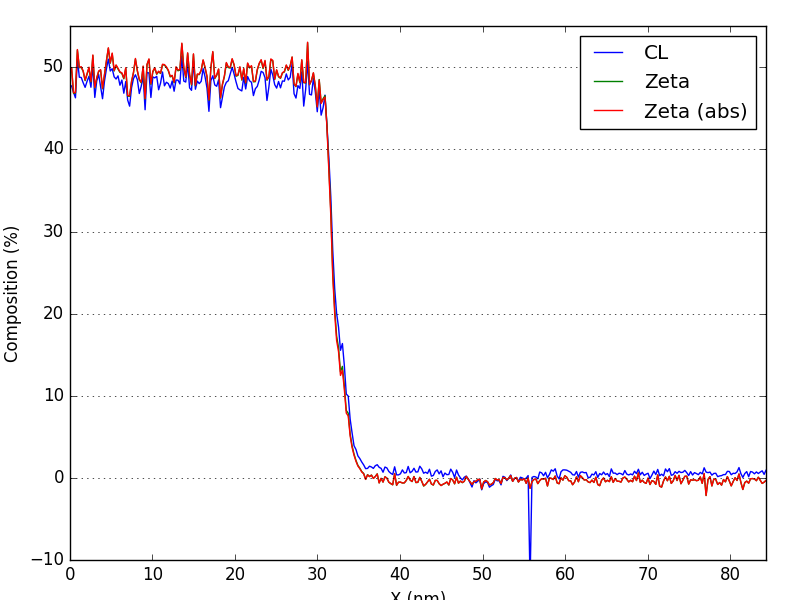
\includegraphics[width=\linewidth]{fig/q-new/oldzetas_Sa_As_Ka}
		\caption{}
		\label{fig:zeta_area1_as}
	\end{subfigure}
\hfill
		\begin{subfigure}{.45\textwidth}
			\centering
			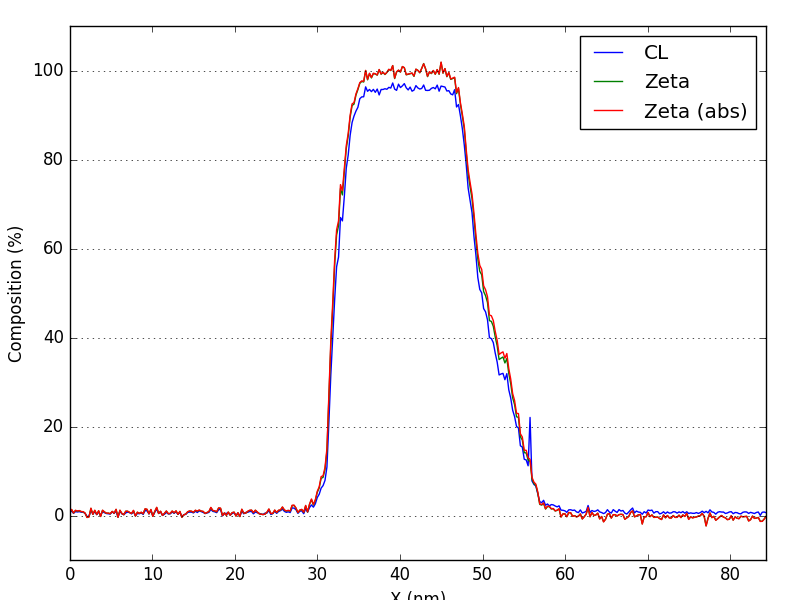
\includegraphics[width=\linewidth]{fig/q-new/oldzetas_Sa_Pd_La}
			\caption{}
			\label{fig:zeta_area1_pd}
		\end{subfigure}%
	\hfill
		\begin{subfigure}{.45\textwidth}
			\centering
			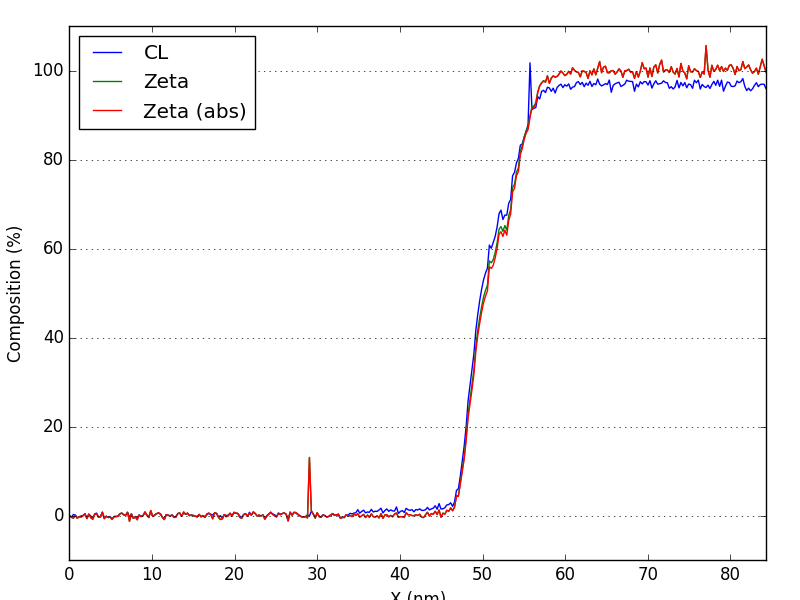
\includegraphics[width=\linewidth]{fig/q-new/oldzetas_Sa_Ge_Ka}
			\caption{}
			\label{fig:zeta_area1_ge}
	\end{subfigure}
\hfill
%		\begin{subfigure}{.5\textwidth}
%			\centering
%			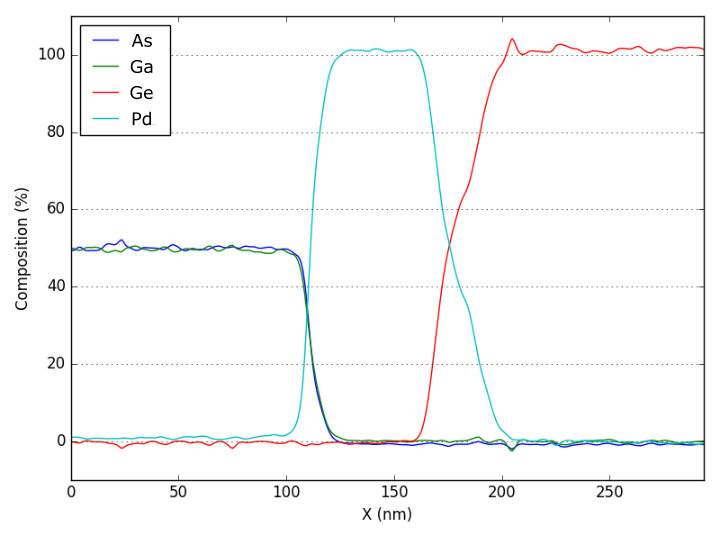
\includegraphics[width=\linewidth]{fig/q/1_all_abscorr4}
%			\caption{}
%			\label{fig:zeta_area1_all}
%	\end{subfigure}%
	\caption{plots of....}
	\label{fig:zeta_area1}
\end{figure}

\begin{figure}
	\begin{subfigure}{.5\textwidth}
		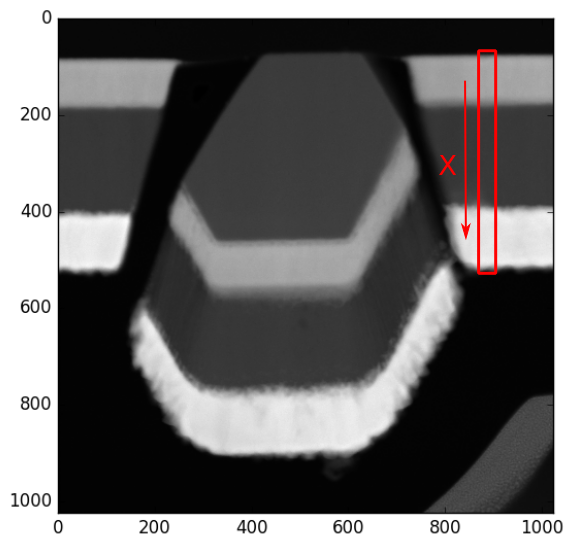
\includegraphics[width=\linewidth]{fig/q/2_overview}
		\caption{Overview}
		\label{fig:zeta_area2_overview}
	\end{subfigure}%
\hfill
	\begin{subfigure}{.5\textwidth}
		\centering
		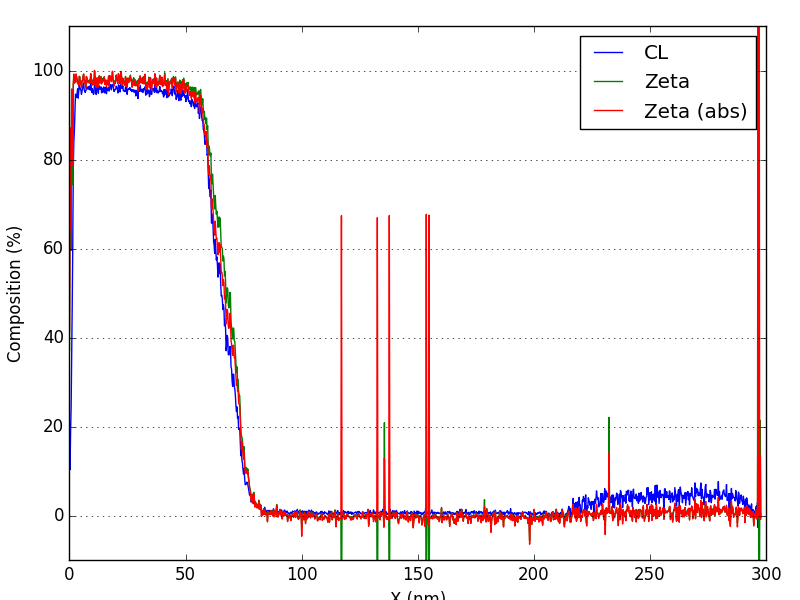
\includegraphics[width=\linewidth]{fig/q-new/oldzetas_Sb_Pd_La}
		\caption{Pd}
		\label{fig:zeta_area2_pd}
	\end{subfigure}
\hfill
	\begin{subfigure}{.5\textwidth}
		\centering
		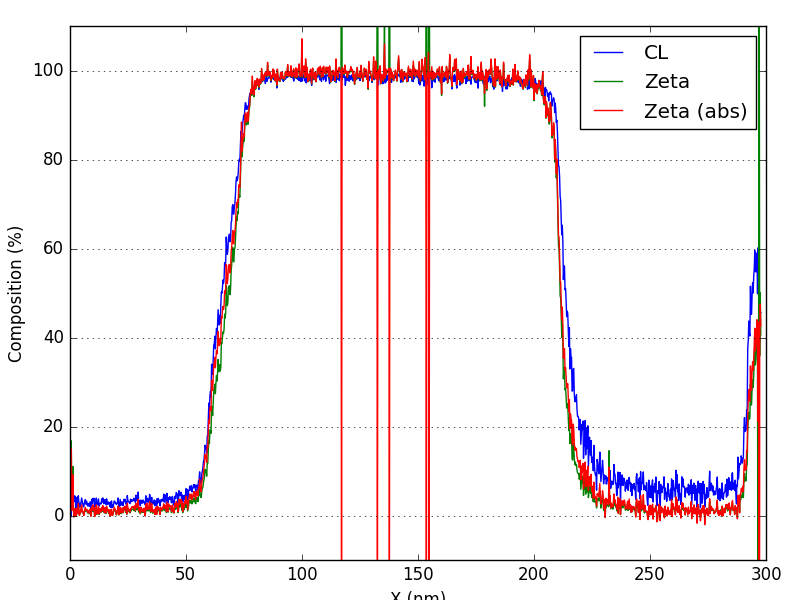
\includegraphics[width=\linewidth]{fig/q-new/oldzetas_Sb_Ge_La}
		\caption{Ge}
		\label{fig:zeta_area2_ge}
	\end{subfigure}%
\hfill
	\begin{subfigure}{.5\textwidth}
		\centering
		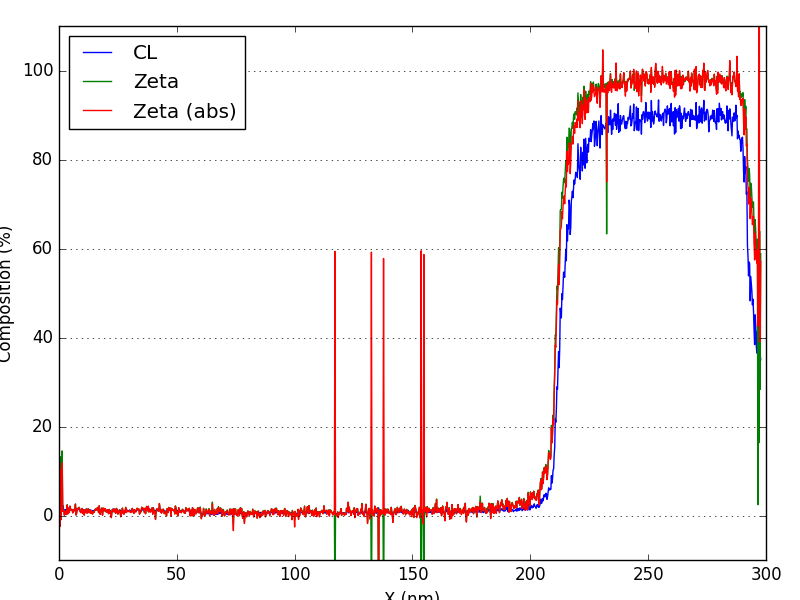
\includegraphics[width=\linewidth]{fig/q-new/oldzetas_Sb_Au_Ma}
		\caption{Au}
		\label{fig:zeta_area2_au}
	\end{subfigure}
%	\begin{subfigure}{.5\textwidth}
%		\centering
%		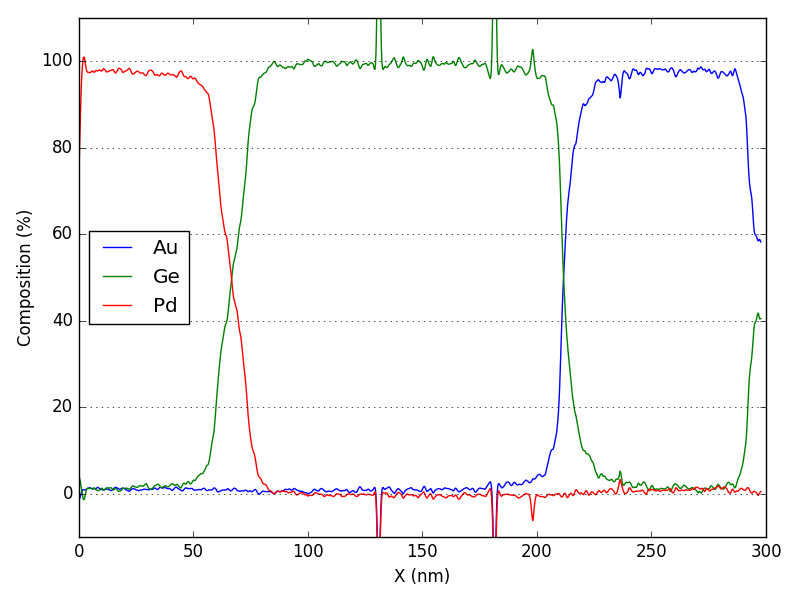
\includegraphics[width=\linewidth]{fig/q/2_all_abscorr2}
%		\caption{All}
%		\label{fig:zeta_area2_all}
%	\end{subfigure}
	\caption{plots of....}
	\label{fig:zeta_area2}
\end{figure}


\begin{figure}
	\centering
	\begin{subfigure}{0.5\linewidth}
		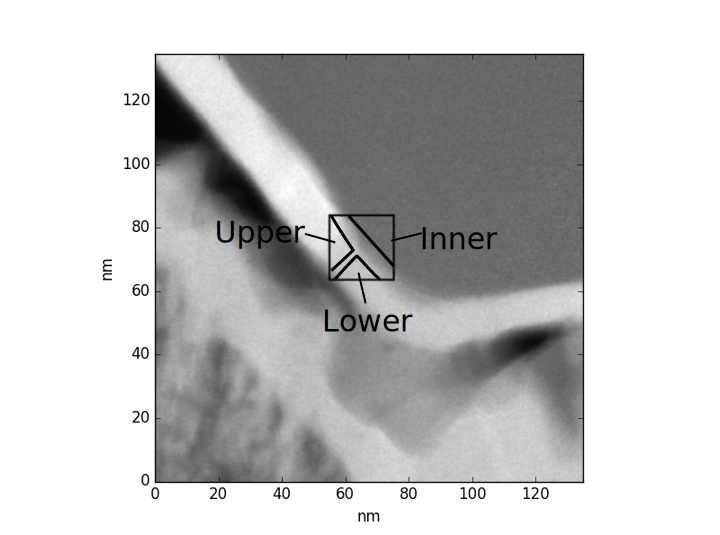
\includegraphics[width=\linewidth]{fig/q/D-E/D}
		\caption{D}
		\label{fig:D-overview}
	\end{subfigure}%
	\hfill
	\begin{subfigure}{0.45\linewidth}
		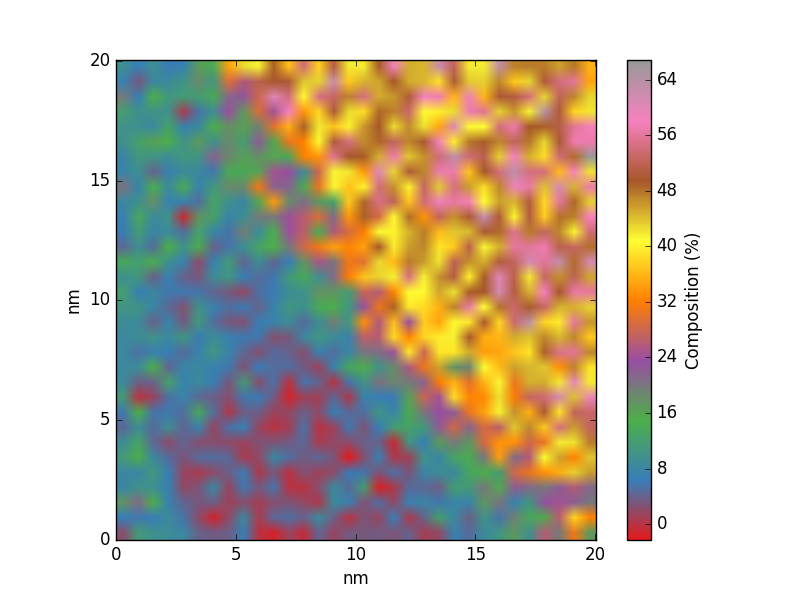
\includegraphics[width=\linewidth]{fig/q-new/D/oldzeta/As_zeta}
		\caption{As}
		\label{fig:Das}
	\end{subfigure}
	\hfill
	\begin{subfigure}{0.45\linewidth}
		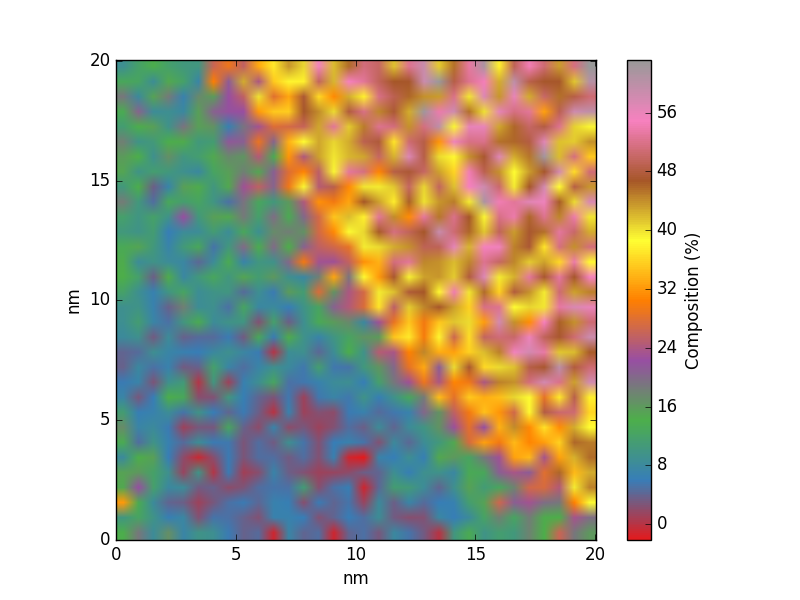
\includegraphics[width=\linewidth]{fig/q-new/D/oldzeta/Ga_zeta}
		\caption{Ga}
		\label{fig:Dga}
	\end{subfigure}%
	\hfill
	\begin{subfigure}{0.45\textwidth}	
		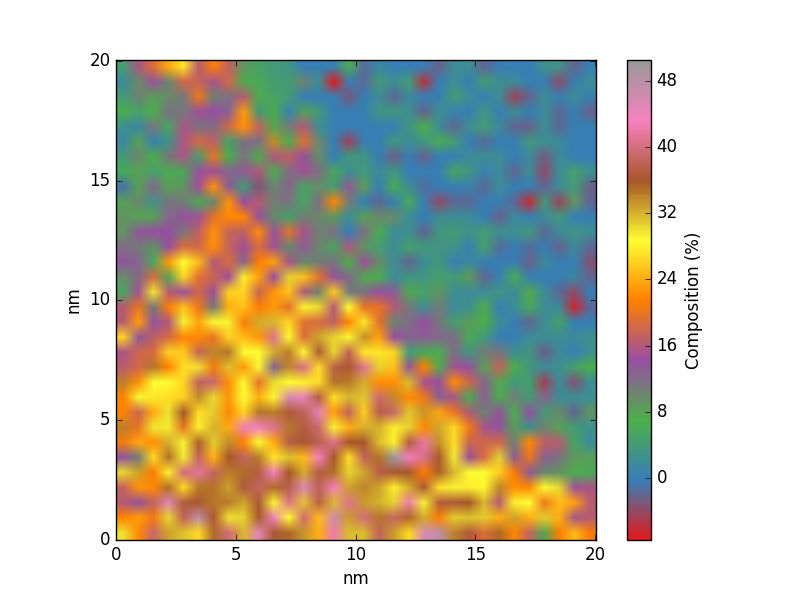
\includegraphics[width=\textwidth]{fig/q-new/D/oldzeta/Ge_zeta}
		\caption{Ge}
		\label{fig:Dge}
	\end{subfigure}
	\hfill
	\begin{subfigure}{0.45\textwidth}
		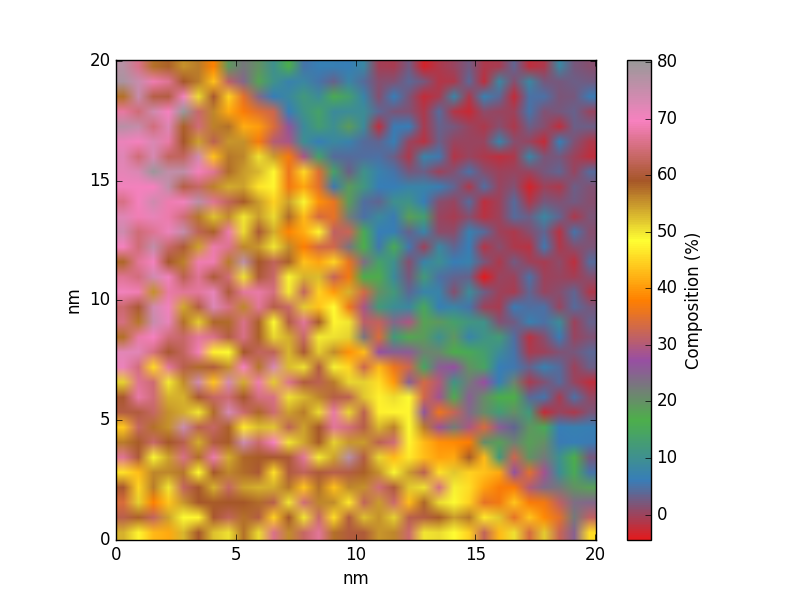
\includegraphics[width=\textwidth]{fig/q-new/D/oldzeta/Pd_zeta}
		\caption{Pd}
		\label{fig:Dpd}
	\end{subfigure}%
\hfill
%	\begin{subfigure}{0.45\textwidth}
%		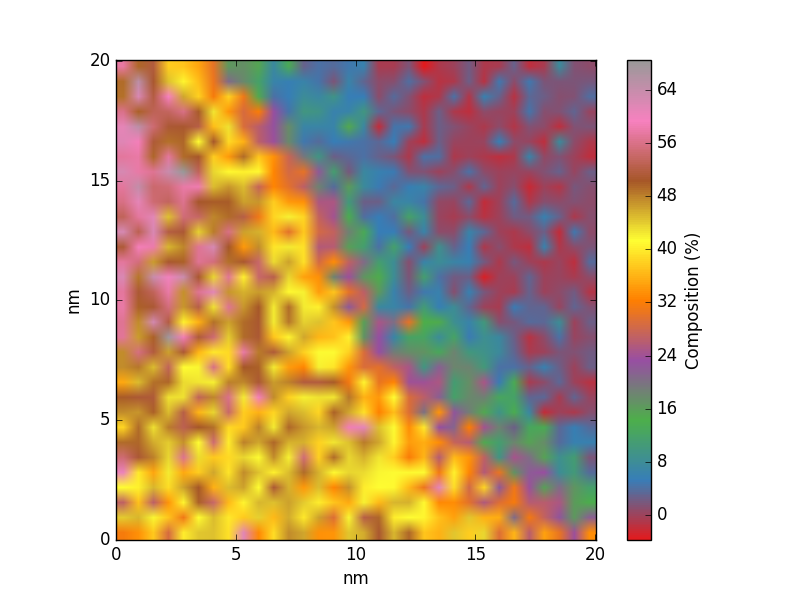
\includegraphics[width=\textwidth]{fig/q-new/D/oldzeta-Au/Pd_zeta}
%		\caption{Pd2}
%		\label{fig:Dpd2}
%	\end{subfigure}%
	\begin{subfigure}{0.45\textwidth}
		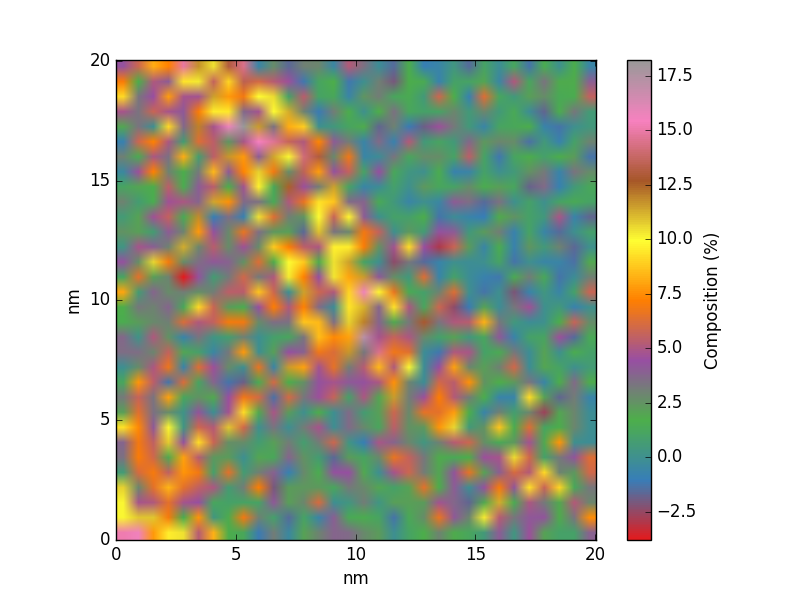
\includegraphics[width=\textwidth]{fig/q-new/D/oldzeta-Au/Au_zeta}
		\caption{Au}
		\label{fig:Dau}
	\end{subfigure}
	\caption{plots of....}
	\label{fig:D}
\end{figure}

\begin{figure}
	\centering
		\begin{subfigure}{0.5\textwidth}
		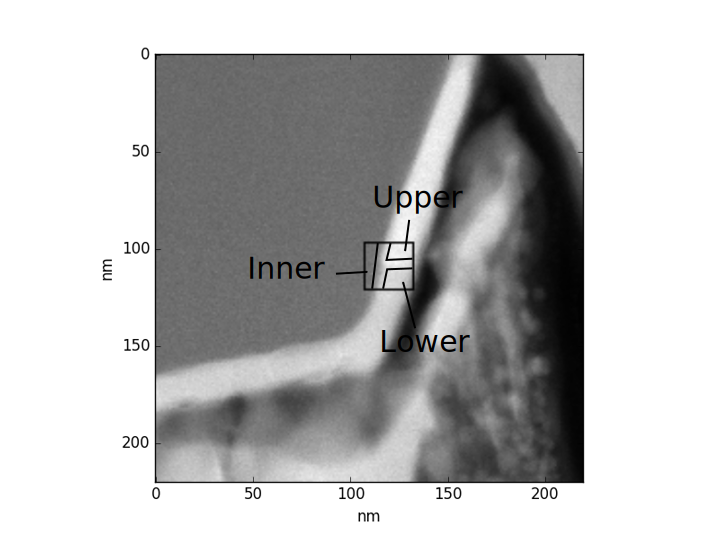
\includegraphics[width=\textwidth]{fig/q/D-E/E}
		\caption{E}
		\label{fig:E-overview}
	\end{subfigure}%
	\hfill
	\begin{subfigure}{0.45\textwidth}
		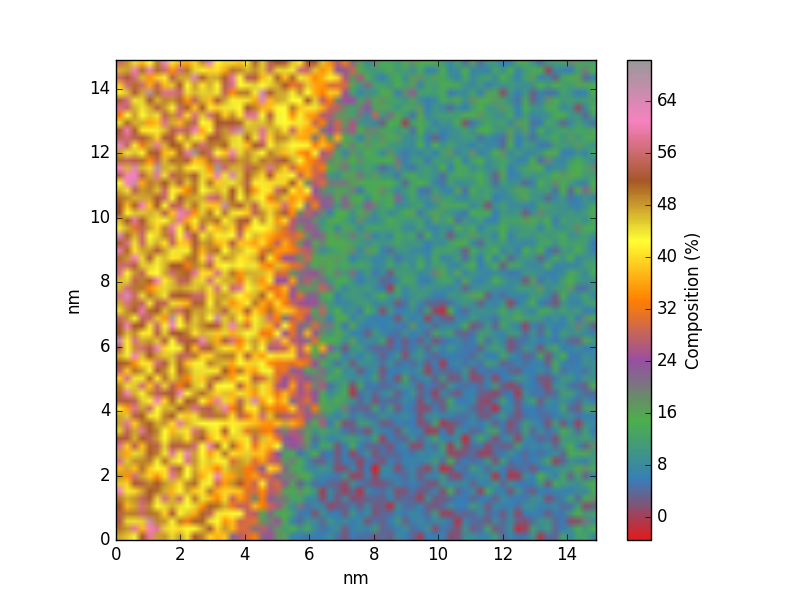
\includegraphics[width=\textwidth]{fig/q-new/E/oldzeta/As_zeta}
		\caption{As}
		\label{fig:Eas}
	\end{subfigure}
	\centering
	\begin{subfigure}{0.45\textwidth}
		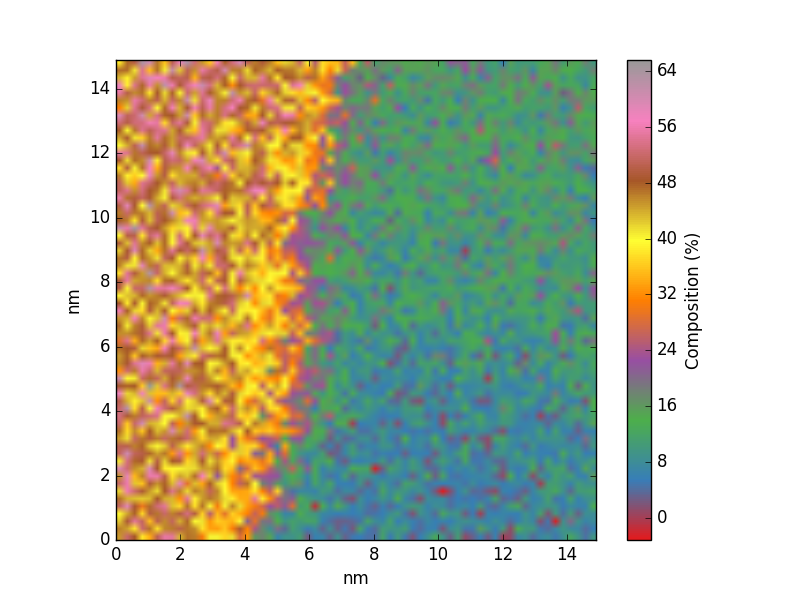
\includegraphics[width=\textwidth]{fig/q-new/E/oldzeta/Ga_zeta}
		\caption{Ga}
		\label{fig:Ega}
	\end{subfigure}%
	\hfill
	\begin{subfigure}{0.45\textwidth}
		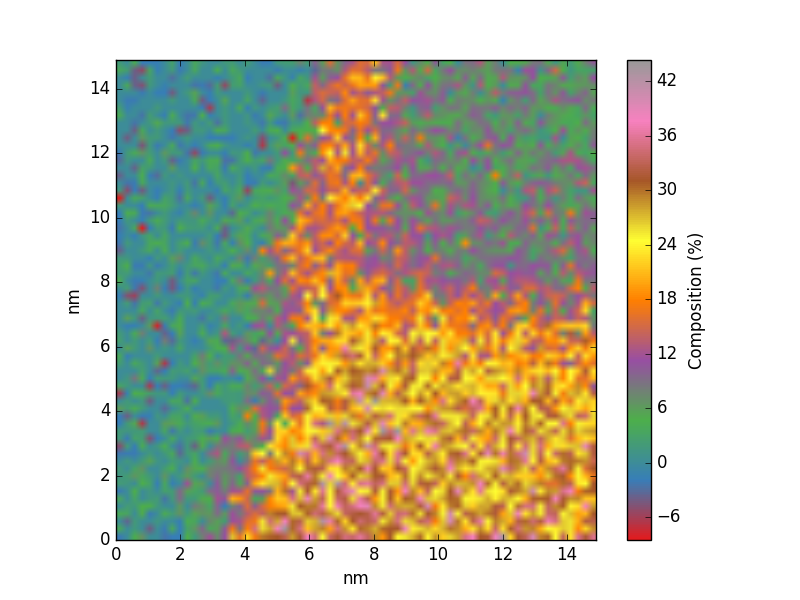
\includegraphics[width=\textwidth]{fig/q-new/E/oldzeta/Ge_zeta}
		\caption{Ge}
		\label{fig:Ege}
	\end{subfigure}
	\begin{subfigure}{0.45\textwidth}
		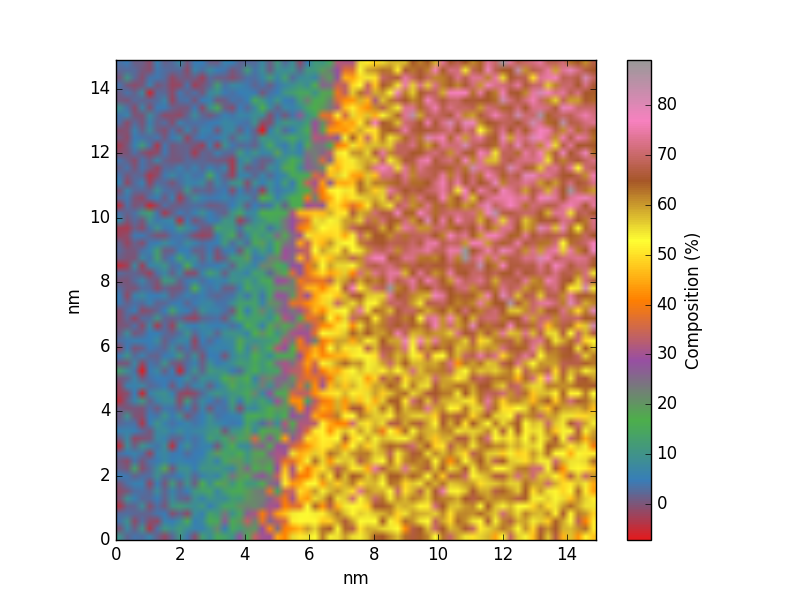
\includegraphics[width=\textwidth]{fig/q-new/E/oldzeta/Pd_zeta}
		\caption{Pd}
		\label{fig:Epd}
	\end{subfigure}%
\hfill
%	\begin{subfigure}{0.45\textwidth}
%		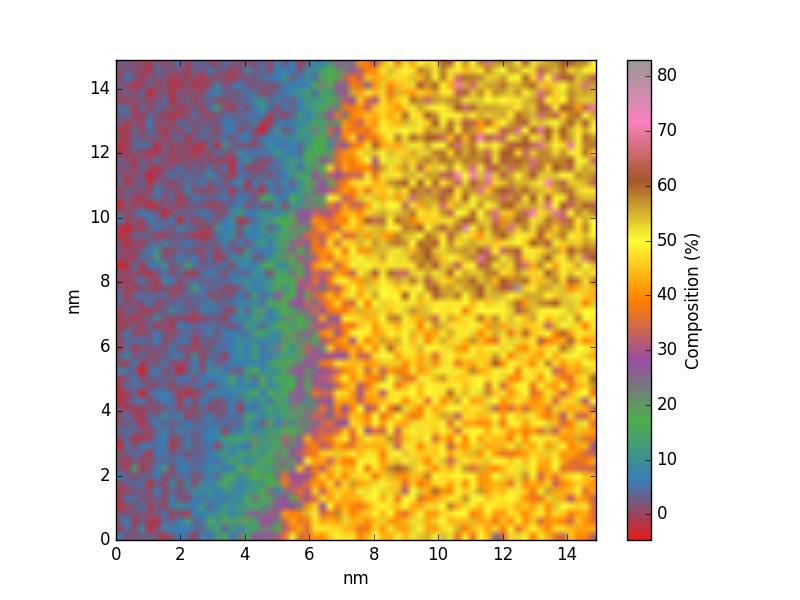
\includegraphics[width=\textwidth]{fig/q-new/E/oldzeta-Au/Pd_zeta}
%		\caption{Pd2}
%		\label{fig:Epd2}
%	\end{subfigure}%
	\begin{subfigure}{0.45\textwidth}
		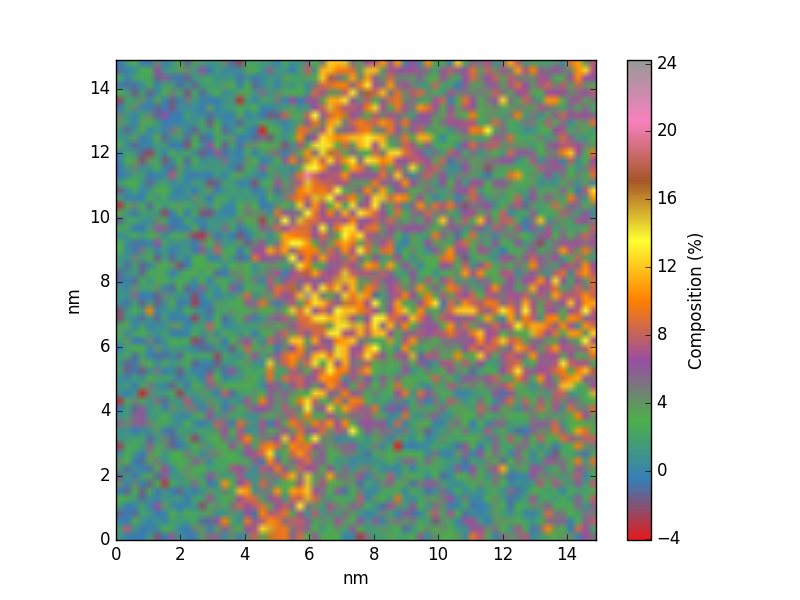
\includegraphics[width=\textwidth]{fig/q-new/E/oldzeta-Au/Au_zeta}
		\caption{Au}
		\label{fig:Eau}
	\end{subfigure}
	\caption{plots of....}
	\label{fig:E}
\end{figure}

The resulting compositions from areas D and E in the heat-treated sample, using the $\zeta$-factor method without absorption correction, are shown in \cref{fig:D,fig:E}. The areas D and E are located, as seen in \cref{fig:D-overview,fig:E-overview}, in the melted region on the left and right side of the nanowire, respectively. As previously explained, it was not possible to get accurate compositions of all elements simultaneously. Therefore, the quantification was done in two stages. The first time with Ga, As, Ge and Pd, using the $K_\alpha$-peaks for Ga, As and Ge, and the $L_\alpha$-peak for Pd. As seen in \cref{fig:spectrum-with-info}, this gives clear and distinct peaks for all the element, and is therefore expected to give accurate results. The second time was performed using all the elements, but now with the $L_\alpha$-lines for Ga, As, Ge and Pd, and the $M_\alpha$-line for Au. This causes a high degree of overlap between the Ga-, As- and Ge-lines, and will therefore overestimate the composition of these elements compared to Pd and Au. These results are therefore not included except for Au, in order to give an indication of the measured composition. \cref{fig:Das,fig:Dga,fig:Dge,fig:Dpd,fig:Eas,fig:Ega,fig:Ege,fig:Epd} are calculated using the first method, while \cref{fig:Dau,fig:Eau} are from the second method.

\cref{tab:D-composition,tab:E-composition} provides a summary of the compositions of areas D and E, respectively, in which the areas have been roughly divided into three regions, as shown in \cref{fig:D-overview,fig:E-overview}. Maps showing the compositions calculated using the CL-method and the $\zeta$-factor with absorption correction are given in \ref{sec:appendix?}. The results from the $\zeta$-factor with absorption correction were mostly very similar to the ones without absorption correction (with a maximum deviation of about 1 pp.), while the CL-method caused offsets by up to 12pp. 
%The results from the CL-method differed from the $\zeta$-method by up to 7-8 pp.

%From \cref{fig:Das,fig:Dga,fig:Dge}, it is seen that the upper right region, which is the left edge of the nanowire, consists of roughly 35-45\% Ga and 35-45\% As, with the remaining 10-25\% being Ge and 0-5\% Pd. \cref{fig:Dge,fig:Dpd} shows that the lower left region consists of 40-50\% Ge, 40-50\% Pd, as well as about 5\% Ga and 5\% As. The upper left region consists of about 60-65\% Pd, 15-20\% Ge and about 10\% Ga and 10\% As. Likewise, \cref{fig:Eas,fig:Ega,fig:Ege} shows approximately the same composition on the left side (the right edge of the nanowire) as the right side in \cref{fig:D}. From looking at \cref{fig:Epd} as well, the upper right area consists of about 65-70\% Pd, 10-15\% Ge and about 10\% Ga and 10\% As, while the lower right consists of about 40-50\% Ge, 40-45\% Pd and 5\% Ga and 5\% As. These results are summarized in \cref{tab:D-E-composition}.

%\begin{table}
%	\caption{For area D (zeta). Parentheses: abs correction}
%	\begin{center}
%		\begin{tabular}{r|cccccc}			
%			Area & Ga & As & Ge & Pd (1) & X Pd (2) & Au\\ 
%			\midrule
%			\hline
%			Inner & 40-60 & 40-60 & 0-7 & 0-7 & X 0-7 & 0-2\\
%			Lower & 3-10& 3-10 & 30-40 & 50-60 & X 40-50 (35-45) & 0-4\\
%			Upper & 5-15& 5-15 & 5-18 & 65-80 & X 55-65 (45-55) & 2-6\\
%			\hline
%		\end{tabular} 
%	\end{center}
%	\label{tab:D-composition}
%\end{table}

\begin{table}
	\caption{For area D (zeta). Parentheses: abs correction}
	\begin{center}
		\begin{tabular}{r|ccccc}			
			Area & Ga & As & Ge & Pd & Au\\ 
			\midrule
			\hline
			Inner & 40-60 & 40-60 & 0-7 & 0-7 & 0-2\\
			Lower & 3-10& 3-10 & 30-40 & 50-60 & 0-4\\
			Upper & 5-15& 5-15 & 5-18 & 65-80 & 2-6\\
			\hline
		\end{tabular} 
	\end{center}
	\label{tab:D-composition}
\end{table}

\begin{table}
	\caption{For area E (zeta). Parentheses: abs correction}
	\begin{center}
		\begin{tabular}{r|ccccc}			
			Area & Ga & As & Ge & Pd & Au\\ 
			\midrule
			\hline
			Inner& 40-60 & 40-60 & 0-5 & 0-10 & 0-2\\
			Lower& 0-10 & 0-10 & 25-35 & 50-60 & 0-6\\
			Upper& 5-15 & 5-15 & 5-12 & 65-80 & 2-10\\
			\hline
		\end{tabular} 
	\end{center}
	\label{tab:E-composition}
\end{table}

%\begin{table}
%	\caption{For area E (zeta). Parentheses: abs correction}
%	\begin{center}
%		\begin{tabular}{r|cccccc}			
%			Area & Ga & As & Ge & $\mathrm{Pd}_1$ & X $\mathrm{Pd}_2$ & Au\\ 
%			\midrule
%			\hline
%			Inner& 40-60 & 40-60 & 0-5 & 0-10 & X 0-10 & 0-2\\
%			Lower& 0-10 & 0-10 & 25-35 & 50-60 & X 40-50 (30-45) & 0-6\\
%			Upper& 5-15 & 5-15 & 5-12 & 65-80 & X 50-70 (40-60) & 2-10\\
%			\hline
%		\end{tabular} 
%	\end{center}
%	\label{tab:E-composition}
%\end{table}


\cref{fig:BCF-overview} shows three areas whose average compositions were calculated using all three techniques, and again two separate calculations were performed. \cref{fig:BCF1} shows the results when using the $K_\alpha$ peaks of Ga, As and Ge, and the $L_\alpha$-peak of Pd, while \cref{fig:BCF2} was calculated using the $L_\alpha$ peaks of Ge and Pd, and the $M_\alpha$-peak of Au. The latter calculation was performed using the $L_\alpha$-lines of Ga and As as well, but this calculation gave compositions of 10-15\% As and 5-10\% Ga in all areas, which is clearly not consistent with \cref{fig:BCF1}, which is also assumed to give more accurate results for Ga and As due to less peak overlap. The figures also shows the standard deviations of the calculated compositions.

\begin{figure}[h!]
	\centering
	\begin{subfigure}{.7\textwidth}
		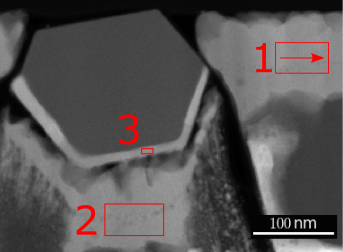
\includegraphics[width=\textwidth]{fig/q/B-C-F/BCF}
		\caption{}
		\label{fig:BCF-overview}
	\end{subfigure}
	\hfill
	\begin{subfigure}{0.7\textwidth}
		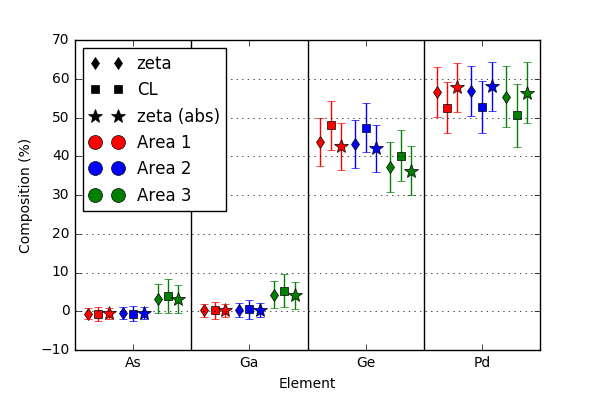
\includegraphics[width=\textwidth]{fig/q/B-C-F/AsGaGePd-GeKline-std}
		\caption{}
		\label{fig:BCF1}
	\end{subfigure}
	\hfill
	\begin{subfigure}{0.7\textwidth}
		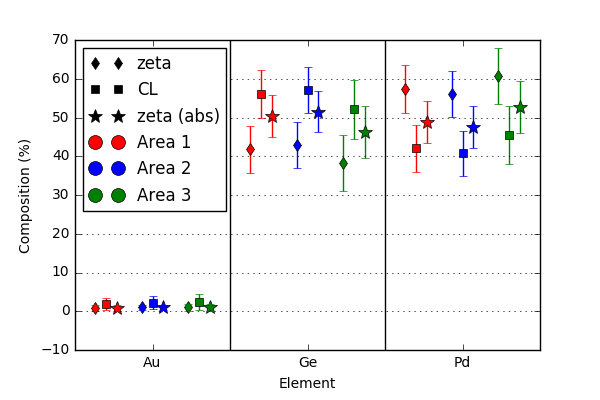
\includegraphics[width=\textwidth]{fig/q/B-C-F/AuGePd-std}
		\caption{}
		\label{fig:BCF2}
	\end{subfigure}
	\caption{
		\label{fig:BCF}%
		Caption}
\end{figure}

It is clear from \cref{fig:BCF1} that areas 1 and 2 contain no Ga or As, while area 3 contains about 5\% of each, and the three different methods give very similar results for these elements. For Ge and Pd, the $\zeta$-methods with and without absorption correction both give a composition of about 40-45 \% Ge and 55-60 \% Pd for areas 1 and 2, and 35-40\% Ge and 55-60 \% Pd for area 3. The CL-method results in approximately 5 pp more Ge and 5 pp less Pd in all areas, compared to the $\zeta$-methods. The differences between the $\zeta$-method with and without absorption correction are consistently only about 1-2 pp.

\cref{fig:BCF2} gives slightly different results. It must here be noted that these results will be very inaccurate for area 3, which from \cref{fig:BCF1} contains Ga and As, which is not included in this quantification process. Both $\zeta$-methods now report little or no presence of Au in all areas, while the CL method gives a few percent. In areas 1 and 2, both the CL-method and the $\zeta$-method with absorption correction reports that the ratios of Ge to Pd have been offset by up to more than 10 pp, compared to \cref{fig:BCF1}. On the other hand, the $\zeta$-method without absorption gives approximately the same values for Ge and Pd; the Ge:Pd ratio has been skewed by a few percent at most.



%\begin{figure}
%	\centering
%	\begin{subfigure}{0.5\textwidth}
%		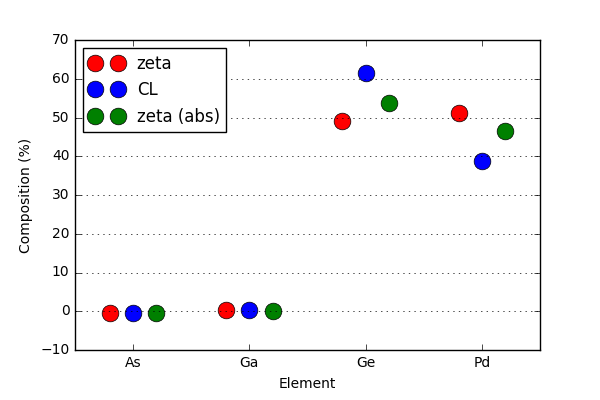
\includegraphics[width=\textwidth]{fig/q/B-C-F/B3}
%		\caption{B - 1}
%		\label{fig:BCF-plots-B}
%	\end{subfigure}%
%	\hfill
%	\begin{subfigure}{0.5\textwidth}
%		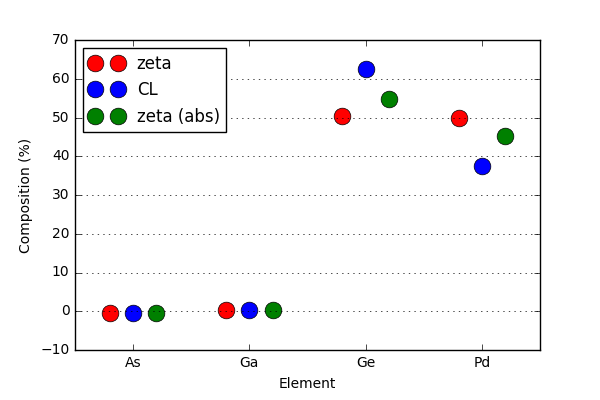
\includegraphics[width=\textwidth]{fig/q/B-C-F/C3}
%		\caption{C - 2}
%		\label{fig:BCF-plots-C}
%	\end{subfigure}
%	\begin{subfigure}{0.5\textwidth}
%	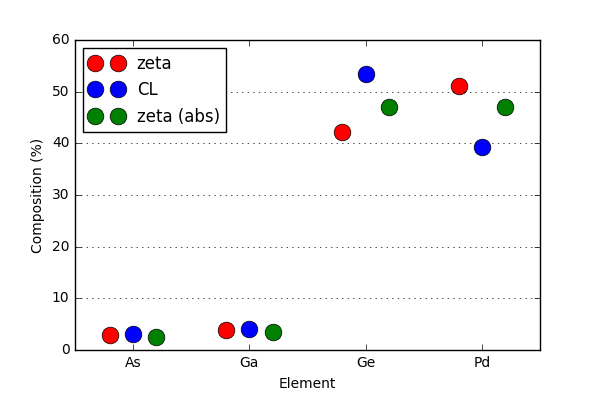
\includegraphics[width=\textwidth]{fig/q/B-C-F/F3}
%	\caption{F - 3}
%	\label{fig:BCF-plots-F}
%	\end{subfigure}%
%	\hfill
%	\begin{subfigure}{0.5\textwidth}
%		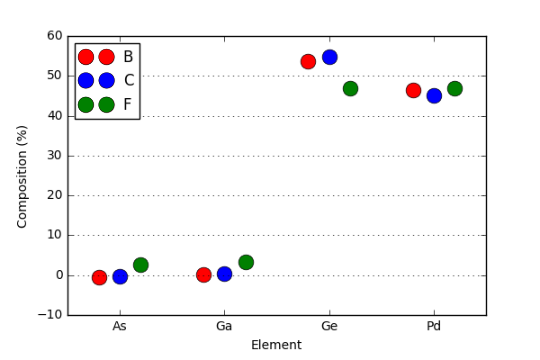
\includegraphics[width=\textwidth]{fig/q/B-C-F/all4}
%		\caption{}
%		\label{fig:BCF-plots-all}
%	\end{subfigure}
%	\caption{
%		\label{fig:BCF-plots}%
%		Caption}
%\end{figure}

